\documentclass[11pt,a4paper]{report}

% ============================================================================
% PACKAGES
% ============================================================================
\usepackage[utf8]{inputenc}
\usepackage[T1]{fontenc}
\usepackage[margin=1in]{geometry}
\usepackage{graphicx}
\usepackage{xcolor}
\usepackage{titlesec}
\usepackage{titletoc}
\usepackage{fancyhdr}
\usepackage{enumitem}
\usepackage{booktabs}
\usepackage{longtable}
\usepackage{tabularx}
\usepackage{multirow}
\usepackage{hyperref}
\usepackage{tcolorbox}
\usepackage{tikz}
\usepackage{pgfplots}
\usepackage{array}
\usepackage{colortbl}
\usepackage{pifont}
\usepackage{parskip}
\usepackage{caption}
\usepackage{float}

\pgfplotsset{compat=1.18}
\usetikzlibrary{shapes.geometric, arrows, positioning, calc, decorations.pathreplacing}

% ============================================================================
% COLOR DEFINITIONS
% ============================================================================
\definecolor{primaryblue}{RGB}{0, 82, 147}
\definecolor{secondaryblue}{RGB}{0, 120, 190}
\definecolor{accentorange}{RGB}{255, 140, 0}
\definecolor{lightgray}{RGB}{245, 245, 245}
\definecolor{darkgray}{RGB}{64, 64, 64}
\definecolor{successgreen}{RGB}{40, 167, 69}
\definecolor{awsorange}{RGB}{255, 153, 0}
\definecolor{azureblue}{RGB}{0, 120, 215}
\definecolor{gcpgreen}{RGB}{52, 168, 83}
\definecolor{snowflakeblue}{RGB}{41, 128, 185}

% ============================================================================
% TCOLORBOX DEFINITIONS
% ============================================================================
\tcbuselibrary{skins,breakable}

\newtcolorbox{objectivebox}{
    colback=primaryblue!5,
    colframe=primaryblue,
    fonttitle=\bfseries,
    title=Learning Objectives,
    breakable,
    left=5pt,
    right=5pt,
    top=5pt,
    bottom=5pt
}

\newtcolorbox{keyconceptbox}{
    colback=accentorange!10,
    colframe=accentorange,
    fonttitle=\bfseries,
    title=Key Concepts,
    breakable,
    left=5pt,
    right=5pt
}

\newtcolorbox{readingbox}{
    colback=successgreen!5,
    colframe=successgreen,
    fonttitle=\bfseries,
    title=Required Reading,
    breakable,
    left=5pt,
    right=5pt
}

\newtcolorbox{labbox}{
    colback=secondaryblue!5,
    colframe=secondaryblue,
    fonttitle=\bfseries,
    title=Hands-On Lab,
    breakable,
    left=5pt,
    right=5pt
}

\newtcolorbox{notebox}{
    colback=lightgray,
    colframe=darkgray,
    fonttitle=\bfseries,
    title=Important Note,
    breakable,
    left=5pt,
    right=5pt
}

\newtcolorbox{assessmentbox}{
    colback=primaryblue!8,
    colframe=primaryblue!80,
    fonttitle=\bfseries,
    breakable,
    left=5pt,
    right=5pt
}

% ============================================================================
% TITLE FORMATTING
% ============================================================================
\titleformat{\chapter}[display]
{\normalfont\huge\bfseries\color{primaryblue}}
{\chaptertitlename\ \thechapter}{20pt}{\Huge}

\titleformat{\section}
{\normalfont\Large\bfseries\color{secondaryblue}}
{\thesection}{1em}{}

\titleformat{\subsection}
{\normalfont\large\bfseries\color{darkgray}}
{\thesubsection}{1em}{}

\titleformat{\subsubsection}
{\normalfont\normalsize\bfseries\color{darkgray}}
{\thesubsubsection}{1em}{}

% ============================================================================
% HEADER/FOOTER
% ============================================================================
\pagestyle{fancy}
\fancyhf{}
\fancyhead[L]{\leftmark}
\fancyhead[R]{\textcolor{primaryblue}{Cloud FinOps Professional Curriculum}}
\fancyfoot[C]{\thepage}
\renewcommand{\headrulewidth}{0.5pt}
\renewcommand{\footrulewidth}{0.3pt}

% ============================================================================
% HYPERREF SETUP
% ============================================================================
\hypersetup{
    colorlinks=true,
    linkcolor=primaryblue,
    urlcolor=secondaryblue,
    citecolor=darkgray,
    pdftitle={Cloud FinOps Professional Curriculum},
    pdfauthor={Cloud FinOps Training Program},
    pdfsubject={Comprehensive FinOps Training Curriculum}
}

% ============================================================================
% CUSTOM COMMANDS
% ============================================================================
\newcommand{\cloudicon}[1]{%
    \ifcase#1\relax
    \or \textcolor{awsorange}{\textbf{AWS}}%
    \or \textcolor{azureblue}{\textbf{Azure}}%
    \or \textcolor{gcpgreen}{\textbf{GCP}}%
    \or \textcolor{snowflakeblue}{\textbf{SF}}%
    \fi
}

\newcommand{\checkmark}{\textcolor{successgreen}{\ding{51}}}
\newcommand{\duration}[1]{\textcolor{darkgray}{$\triangleright$ #1}}
\newcommand{\difficulty}[1]{\textcolor{accentorange}{[#1]}}

% ============================================================================
% DOCUMENT BEGIN
% ============================================================================
\begin{document}

% ============================================================================
% TITLE PAGE
% ============================================================================
\begin{titlepage}
    \centering
    \vspace*{1cm}
    
    \begin{tikzpicture}[remember picture, overlay]
        \fill[primaryblue] (current page.north west) rectangle ([yshift=-4cm]current page.north east);
    \end{tikzpicture}
    
    \vspace{1cm}
    
    {\Huge\bfseries\textcolor{primaryblue}{Cloud FinOps}\\[0.5cm]}
    {\Huge\bfseries\textcolor{secondaryblue}{Professional Curriculum}\\[1cm]}
    
    \vspace{0.5cm}
    
    {\Large A Comprehensive Training Program for\\[0.3cm]
    Cloud Financial Management Excellence\\[2cm]}
    
    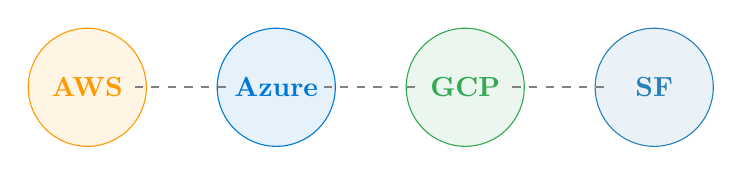
\begin{tikzpicture}[scale=0.8]
        % AWS Icon
        \node[circle, draw=awsorange, fill=awsorange!10, minimum size=1.5cm] at (0,0) {\textcolor{awsorange}{\textbf{AWS}}};
        % Azure Icon
        \node[circle, draw=azureblue, fill=azureblue!10, minimum size=1.5cm] at (3,0) {\textcolor{azureblue}{\textbf{Azure}}};
        % GCP Icon
        \node[circle, draw=gcpgreen, fill=gcpgreen!10, minimum size=1.5cm] at (6,0) {\textcolor{gcpgreen}{\textbf{GCP}}};
        % Snowflake Icon
        \node[circle, draw=snowflakeblue, fill=snowflakeblue!10, minimum size=1.5cm] at (9,0) {\textcolor{snowflakeblue}{\textbf{SF}}};
        
        % Connecting lines
        \draw[thick, gray, dashed] (0.75,0) -- (2.25,0);
        \draw[thick, gray, dashed] (3.75,0) -- (5.25,0);
        \draw[thick, gray, dashed] (6.75,0) -- (8.25,0);
    \end{tikzpicture}
    
    \vspace{2cm}
    
    {\large\textcolor{darkgray}{Curriculum Version 1.0}\\[0.5cm]}
    {\large\textcolor{darkgray}{2025 Edition}\\[2cm]}
    
    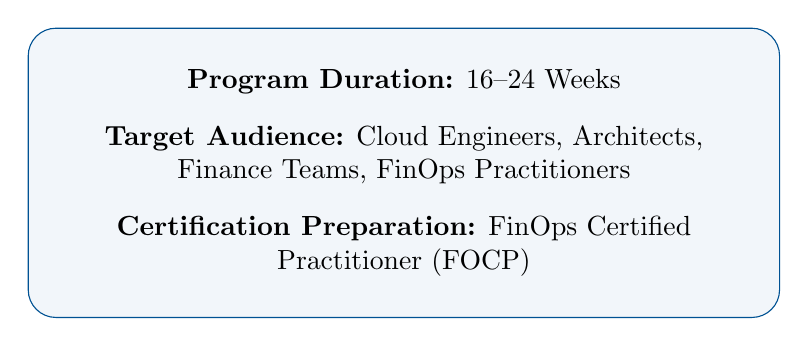
\begin{tikzpicture}
        \node[draw=primaryblue, rounded corners=10pt, inner sep=15pt, fill=primaryblue!5] {
            \begin{minipage}{0.7\textwidth}
                \centering
                \textbf{Program Duration:} 16--24 Weeks\\[0.3cm]
                \textbf{Target Audience:} Cloud Engineers, Architects, Finance Teams, FinOps Practitioners\\[0.3cm]
                \textbf{Certification Preparation:} FinOps Certified Practitioner (FOCP)
            \end{minipage}
        };
    \end{tikzpicture}
    
    \vfill
    
\end{titlepage}

% ============================================================================
% TABLE OF CONTENTS
% ============================================================================
\tableofcontents
\newpage

% ============================================================================
% CHAPTER 1: PROGRAM OVERVIEW
% ============================================================================
\chapter{Program Overview}

\section{Executive Summary}

Cloud FinOps represents a transformative discipline that brings financial accountability to the variable spend model of cloud computing. This comprehensive curriculum is designed to develop practitioners who can effectively manage, optimize, and govern cloud financial operations across enterprise environments.

This program synthesizes knowledge from the industry's most authoritative texts, including foundational works by J.R. Storment and Mike Fuller, practical implementation guides, and platform-specific optimization strategies. The curriculum follows a progressive learning path from foundational concepts through advanced automation and organizational scaling.

\section{Program Philosophy}

The Cloud FinOps discipline operates at the intersection of technology, finance, and organizational culture. This curriculum embraces three core principles:

\begin{enumerate}[leftmargin=*]
    \item \textbf{Teams must collaborate:} FinOps requires cross-functional alignment between engineering, finance, product, and executive leadership.
    
    \item \textbf{Business value drives decisions:} Every cloud spending decision should be evaluated through the lens of business value creation, not merely cost reduction.
    
    \item \textbf{Everyone takes ownership:} Cloud cost management is a shared responsibility that requires distributed accountability across the organization.
\end{enumerate}

\section{Target Audience}

This curriculum is designed for multiple stakeholder groups:

\begin{table}[H]
\centering
\begin{tabularx}{\textwidth}{>{\bfseries}l X}
\toprule
\textbf{Role Category} & \textbf{Description} \\
\midrule
Cloud Engineers & Practitioners responsible for designing, deploying, and managing cloud infrastructure \\
\addlinespace
DevOps/SRE Teams & Teams managing CI/CD pipelines and operational efficiency \\
\addlinespace
Cloud Architects & Professionals designing enterprise cloud architectures \\
\addlinespace
Finance Teams & Financial analysts and controllers working with cloud budgets \\
\addlinespace
Product Managers & Leaders making cost-aware product decisions \\
\addlinespace
FinOps Practitioners & Dedicated FinOps team members and analysts \\
\addlinespace
IT Leadership & Directors, VPs, and CIOs overseeing cloud strategy \\
\bottomrule
\end{tabularx}
\caption{Target Audience by Role Category}
\end{table}

\section{Prerequisites}

Participants should possess the following foundational knowledge:

\begin{itemize}[leftmargin=*]
    \item Basic understanding of cloud computing concepts (IaaS, PaaS, SaaS)
    \item Familiarity with at least one major cloud platform (AWS, Azure, or GCP)
    \item Understanding of fundamental financial concepts (budgets, forecasting, ROI)
    \item Experience with organizational IT operations or software development
    \item Basic proficiency with spreadsheets and data analysis tools
\end{itemize}

\section{Learning Outcomes}

Upon completion of this curriculum, participants will be able to:

\begin{objectivebox}
\begin{enumerate}[leftmargin=*]
    \item Articulate the FinOps lifecycle (Inform, Optimize, Operate) and apply it to organizational contexts
    \item Design and implement comprehensive cloud cost visibility and allocation strategies
    \item Execute optimization techniques across compute, storage, networking, and data services
    \item Develop forecasting models and anomaly detection systems for cloud spend
    \item Build automated cost governance workflows using cloud-native and third-party tools
    \item Create organizational frameworks for scaling FinOps practices enterprise-wide
    \item Apply platform-specific optimization strategies for AWS, Azure, GCP, and Snowflake
    \item Integrate sustainability considerations into cloud financial management
\end{enumerate}
\end{objectivebox}

\section{Core Textbook Library}

This curriculum is structured around seven authoritative texts that form the FinOps professional's core bookshelf:

\begin{table}[H]
\centering
\small
\begin{tabularx}{\textwidth}{>{\raggedright\arraybackslash}p{4.5cm} >{\raggedright\arraybackslash}p{3cm} X c}
\toprule
\textbf{Title} & \textbf{Authors} & \textbf{Focus Area} & \textbf{Level} \\
\midrule
Cloud FinOps, 2nd Edition & Storment \& Fuller & Foundation \& Culture & \difficulty{Intro--Int} \\
\addlinespace
Efficient Cloud FinOps & San Miguel Sánchez \& Obando García & Multi-Cloud Implementation & \difficulty{Intermediate} \\
\addlinespace
AWS FinOps Simplified & Peter Chung & AWS Platform & \difficulty{Intro--Int} \\
\addlinespace
FinOps Handbook for Microsoft Azure & Maulik Soni & Azure Platform & \difficulty{Intro--Int} \\
\addlinespace
FinOps for Snowflake & Ravi Kumar et al. & Snowflake Platform & \difficulty{Intermediate} \\
\addlinespace
Practical FinOps & Mohamed Labouardy & Automation \& AI/ML & \difficulty{Int--Adv} \\
\addlinespace
Scaling Cloud FinOps & Kanumuri \& Zeier & Organizational Scaling & \difficulty{Int--Adv} \\
\bottomrule
\end{tabularx}
\caption{Core Textbook Library with Difficulty Levels}
\end{table}

\section{Program Structure}

The curriculum is organized into four progressive phases spanning 16--24 weeks:

\begin{figure}[H]
\centering
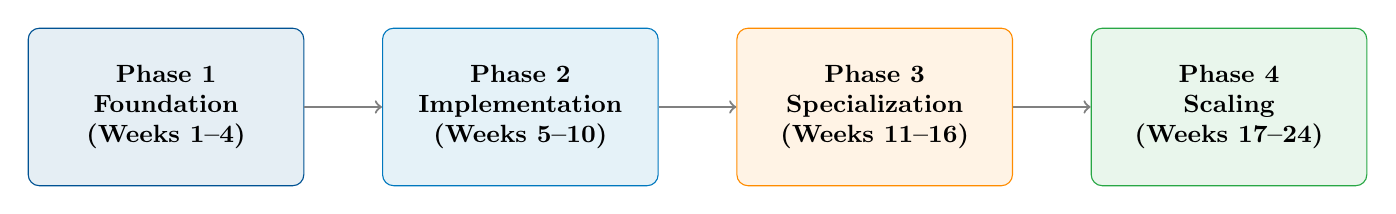
\begin{tikzpicture}[
    phase/.style={rectangle, rounded corners, draw=#1, fill=#1!10, minimum width=3.5cm, minimum height=2cm, align=center, font=\small\bfseries},
    arrow/.style={->, thick, gray}
]
    \node[phase=primaryblue] (p1) at (0,0) {Phase 1\\Foundation\\(Weeks 1--4)};
    \node[phase=secondaryblue] (p2) at (4.5,0) {Phase 2\\Implementation\\(Weeks 5--10)};
    \node[phase=accentorange] (p3) at (9,0) {Phase 3\\Specialization\\(Weeks 11--16)};
    \node[phase=successgreen] (p4) at (13.5,0) {Phase 4\\Scaling\\(Weeks 17--24)};
    
    \draw[arrow] (p1) -- (p2);
    \draw[arrow] (p2) -- (p3);
    \draw[arrow] (p3) -- (p4);
\end{tikzpicture}
\caption{Four-Phase Curriculum Structure}
\end{figure}

% ============================================================================
% CHAPTER 2: PHASE 1 - FOUNDATION
% ============================================================================
\chapter{Phase 1: Foundation and Shared Language}
\thispagestyle{fancy}

\begin{tcolorbox}[colback=primaryblue!5, colframe=primaryblue, title=Phase Overview]
\textbf{Duration:} 4 Weeks \hfill \textbf{Primary Text:} Cloud FinOps, 2nd Edition\\[0.3cm]
\textbf{Objective:} Establish foundational understanding of FinOps principles, lifecycle, and organizational culture
\end{tcolorbox}

\section{Module 1.1: Introduction to Cloud FinOps}

\duration{Week 1} \hfill \difficulty{Introductory}

\subsection{Learning Objectives}

\begin{objectivebox}
Upon completing this module, participants will be able to:
\begin{itemize}[leftmargin=*]
    \item Define Cloud FinOps and articulate its business value proposition
    \item Explain the historical evolution from on-premises cost management to cloud financial operations
    \item Identify the key stakeholders in a FinOps practice and their respective responsibilities
    \item Describe the relationship between FinOps and other IT frameworks (ITIL, DevOps, Agile)
\end{itemize}
\end{objectivebox}

\subsection{Topics Covered}

\subsubsection{What is Cloud FinOps?}

Cloud FinOps (Cloud Financial Operations) is an evolving cloud financial management discipline and cultural practice that enables organizations to get maximum business value by helping engineering, finance, technology, and business teams collaborate on data-driven spending decisions.

\begin{keyconceptbox}
\textbf{Core Definition:} FinOps is an operational framework and cultural shift that brings financial accountability to the variable spend model of cloud, enabling distributed teams to make business trade-offs between speed, cost, and quality.
\end{keyconceptbox}

\subsubsection{The Variable Spend Model Challenge}

Unlike traditional IT procurement with fixed capital expenditures, cloud computing introduces a consumption-based model where costs directly correlate with usage. This shift creates both opportunities and challenges:

\begin{itemize}[leftmargin=*]
    \item \textbf{Opportunities:} Elasticity, pay-per-use efficiency, rapid scaling, reduced upfront investment
    \item \textbf{Challenges:} Cost unpredictability, sprawl, accountability gaps, budget overruns
\end{itemize}

\subsubsection{FinOps Stakeholder Ecosystem}

The FinOps practice requires coordination across multiple organizational functions:

\begin{table}[H]
\centering
\begin{tabularx}{\textwidth}{>{\bfseries}l X X}
\toprule
\textbf{Stakeholder} & \textbf{Primary Concerns} & \textbf{FinOps Contribution} \\
\midrule
Engineering & Performance, reliability, velocity & Cost-aware architecture decisions \\
Finance & Budget accuracy, forecasting, compliance & Cloud-specific financial analysis \\
Product & Feature velocity, user experience & Unit economics understanding \\
Executives & Strategic investment, ROI & Business value alignment \\
Procurement & Vendor management, contracts & Commitment-based discounts \\
\bottomrule
\end{tabularx}
\caption{FinOps Stakeholder Responsibilities Matrix}
\end{table}

\subsection{Required Reading}

\begin{readingbox}
\textbf{Cloud FinOps, 2nd Edition} by Storment \& Fuller
\begin{itemize}[leftmargin=*]
    \item Chapter 1: What is Cloud FinOps?
    \item Chapter 2: Why FinOps?
    \item Part I Introduction: The Cultural Shift
\end{itemize}
\end{readingbox}

\subsection{Hands-On Lab 1.1}

\begin{labbox}
\textbf{Lab: Cloud Spend Discovery Assessment}\\[0.3cm]
\textbf{Objective:} Conduct an initial assessment of your organization's current cloud spend visibility and governance maturity.\\[0.3cm]
\textbf{Activities:}
\begin{enumerate}[leftmargin=*]
    \item Access your organization's cloud billing console (AWS Cost Explorer, Azure Cost Management, or GCP Billing)
    \item Document the current monthly cloud spend across all accounts/subscriptions
    \item Identify the top 10 cost-driving services
    \item Assess current tagging coverage and consistency
    \item Complete the FinOps Maturity Assessment questionnaire
\end{enumerate}
\textbf{Deliverable:} Cloud Spend Discovery Report (2--3 pages)
\end{labbox}

% ============================================================================
% Module 1.2
% ============================================================================
\section{Module 1.2: The FinOps Lifecycle}

\duration{Week 2} \hfill \difficulty{Introductory}

\subsection{Learning Objectives}

\begin{objectivebox}
Upon completing this module, participants will be able to:
\begin{itemize}[leftmargin=*]
    \item Explain the three phases of the FinOps lifecycle: Inform, Optimize, Operate
    \item Describe the iterative nature of FinOps practice maturation
    \item Map organizational activities to appropriate lifecycle phases
    \item Assess current organizational positioning within the lifecycle framework
\end{itemize}
\end{objectivebox}

\subsection{Topics Covered}

\subsubsection{The Inform Phase}

The Inform phase establishes visibility and accountability for cloud costs. This phase focuses on:

\begin{itemize}[leftmargin=*]
    \item \textbf{Cost Allocation:} Tagging strategies, account structures, and chargeback/showback models
    \item \textbf{Visibility:} Dashboards, reports, and real-time cost monitoring
    \item \textbf{Benchmarking:} Internal and external cost comparisons
    \item \textbf{Forecasting:} Predictive models for future spend
\end{itemize}

\subsubsection{The Optimize Phase}

The Optimize phase focuses on reducing waste and maximizing the value of cloud investments:

\begin{itemize}[leftmargin=*]
    \item \textbf{Rightsizing:} Matching resource capacity to actual workload requirements
    \item \textbf{Rate Optimization:} Reserved Instances, Savings Plans, Committed Use Discounts
    \item \textbf{Architectural Optimization:} Serverless, containerization, spot/preemptible instances
    \item \textbf{Waste Elimination:} Identifying and removing unused or orphaned resources
\end{itemize}

\subsubsection{The Operate Phase}

The Operate phase establishes ongoing governance and continuous improvement:

\begin{itemize}[leftmargin=*]
    \item \textbf{Governance:} Policies, guardrails, and approval workflows
    \item \textbf{Automation:} Scheduled actions, auto-scaling, policy enforcement
    \item \textbf{Continuous Improvement:} Regular optimization reviews and process refinement
    \item \textbf{Organizational Alignment:} Cross-functional collaboration and communication
\end{itemize}

\begin{figure}[H]
\centering
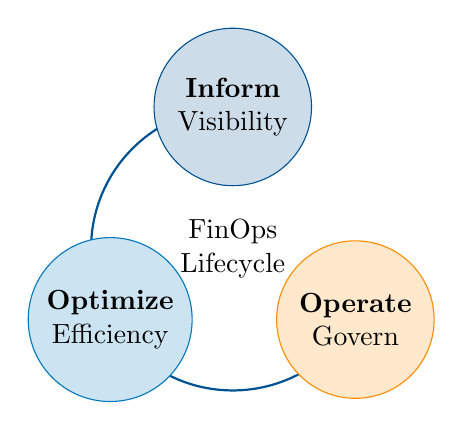
\begin{tikzpicture}[scale=0.9]
    % Circular arrows
    \draw[thick, primaryblue, ->] (0,2) arc (90:350:2);
    
    % Phase nodes
    \node[circle, draw=primaryblue, fill=primaryblue!20, minimum size=2cm, align=center] at (0,2) {\textbf{Inform}\\Visibility};
    \node[circle, draw=secondaryblue, fill=secondaryblue!20, minimum size=2cm, align=center] at (-1.73,-1) {\textbf{Optimize}\\Efficiency};
    \node[circle, draw=accentorange, fill=accentorange!20, minimum size=2cm, align=center] at (1.73,-1) {\textbf{Operate}\\Govern};
    
    % Center
    \node[align=center] at (0,0) {FinOps\\Lifecycle};
\end{tikzpicture}
\caption{The FinOps Lifecycle: Inform, Optimize, Operate}
\end{figure}

\subsection{Required Reading}

\begin{readingbox}
\textbf{Cloud FinOps, 2nd Edition} by Storment \& Fuller
\begin{itemize}[leftmargin=*]
    \item Chapter 3: The FinOps Lifecycle
    \item Chapter 4: Inform Phase Deep Dive
    \item Chapter 5: Optimize Phase Deep Dive
    \item Chapter 6: Operate Phase Deep Dive
\end{itemize}
\end{readingbox}

\subsection{Hands-On Lab 1.2}

\begin{labbox}
\textbf{Lab: Lifecycle Phase Mapping Exercise}\\[0.3cm]
\textbf{Objective:} Map your organization's current FinOps activities to the lifecycle framework and identify gaps.\\[0.3cm]
\textbf{Activities:}
\begin{enumerate}[leftmargin=*]
    \item Create a three-column matrix with Inform, Optimize, and Operate headers
    \item List all current cost management activities in your organization
    \item Categorize each activity into the appropriate lifecycle phase
    \item Identify phases with limited or no activities (gaps)
    \item Propose three high-impact activities for each gap area
\end{enumerate}
\textbf{Deliverable:} Lifecycle Gap Analysis with Recommendations
\end{labbox}

% ============================================================================
% Module 1.3
% ============================================================================
\section{Module 1.3: Anatomy of Cloud Bills}

\duration{Week 3} \hfill \difficulty{Intermediate}

\subsection{Learning Objectives}

\begin{objectivebox}
Upon completing this module, participants will be able to:
\begin{itemize}[leftmargin=*]
    \item Interpret cloud billing structures across AWS, Azure, and GCP
    \item Identify key billing dimensions: services, regions, usage types, pricing models
    \item Understand commitment-based discount mechanisms (RIs, Savings Plans, CUDs)
    \item Recognize common billing anomalies and their root causes
\end{itemize}
\end{objectivebox}

\subsection{Topics Covered}

\subsubsection{Cloud Pricing Model Fundamentals}

Cloud providers employ complex, multi-dimensional pricing models. Understanding these models is essential for effective cost management:

\begin{table}[H]
\centering
\begin{tabularx}{\textwidth}{>{\bfseries}l X X X}
\toprule
\textbf{Dimension} & \textbf{AWS} & \textbf{Azure} & \textbf{GCP} \\
\midrule
On-Demand & Pay-as-you-go & Pay-as-you-go & On-demand \\
Committed & Reserved Instances, Savings Plans & Reserved Instances, Reserved Capacity & Committed Use Discounts \\
Spot/Preemptible & Spot Instances & Spot VMs & Preemptible VMs, Spot VMs \\
Free Tier & 12-month + always free & 12-month + always free & Always free + trial credits \\
\bottomrule
\end{tabularx}
\caption{Pricing Model Comparison Across Major Cloud Providers}
\end{table}

\subsubsection{Bill Anatomy: Key Components}

\begin{itemize}[leftmargin=*]
    \item \textbf{Account/Subscription Structure:} Hierarchical organization affecting consolidated billing
    \item \textbf{Service Categories:} Compute, storage, networking, database, analytics, AI/ML
    \item \textbf{Usage Types:} Instance hours, data transfer, storage GB-months, API calls
    \item \textbf{Pricing Tiers:} Volume-based discounts, tiered pricing models
    \item \textbf{Tax and Support:} Regional taxes, support plan charges
\end{itemize}

\subsubsection{Commitment-Based Discounts Deep Dive}

\begin{notebox}
Commitment-based discounts represent the most significant opportunity for cost optimization, often yielding 30--72\% savings compared to on-demand pricing. However, over-commitment creates waste, making accurate capacity planning essential.
\end{notebox}

\textbf{AWS Reserved Instances and Savings Plans:}
\begin{itemize}[leftmargin=*]
    \item Standard RIs: Up to 72\% discount, specific instance type and region
    \item Convertible RIs: Up to 66\% discount, flexibility to change instance families
    \item Compute Savings Plans: Up to 66\% discount, applies to EC2, Lambda, Fargate
    \item EC2 Instance Savings Plans: Up to 72\% discount, specific instance family and region
\end{itemize}

\textbf{Azure Reserved Instances and Capacity:}
\begin{itemize}[leftmargin=*]
    \item Reserved VM Instances: 1-year or 3-year terms, up to 72\% savings
    \item Azure Hybrid Benefit: Leverage existing Windows Server and SQL licenses
    \item Reserved Capacity: Available for Cosmos DB, SQL Database, Blob Storage
\end{itemize}

\textbf{GCP Committed Use Discounts:}
\begin{itemize}[leftmargin=*]
    \item Committed Use Contracts: 1-year or 3-year, up to 57\% discount
    \item Sustained Use Discounts: Automatic, no commitment required, up to 30\%
    \item Flexible Committed Use: Apply across machine families
\end{itemize}

\subsection{Required Reading}

\begin{readingbox}
\textbf{Cloud FinOps, 2nd Edition} by Storment \& Fuller
\begin{itemize}[leftmargin=*]
    \item Chapter 7: The Anatomy of the Cloud Bill
    \item Chapter 8: Understanding Pricing Models
\end{itemize}
\textbf{Efficient Cloud FinOps} by San Miguel Sánchez \& Obando García
\begin{itemize}[leftmargin=*]
    \item Chapter 2: Cloud Cost Fundamentals (AWS, Azure, GCP sections)
\end{itemize}
\end{readingbox}

\subsection{Hands-On Lab 1.3}

\begin{labbox}
\textbf{Lab: Bill Anatomy Deep Dive}\\[0.3cm]
\textbf{Objective:} Analyze a real cloud bill to understand cost drivers and identify optimization opportunities.\\[0.3cm]
\textbf{Activities:}
\begin{enumerate}[leftmargin=*]
    \item Export detailed billing data (AWS Cost and Usage Report, Azure Cost Export, or GCP Billing Export)
    \item Load data into a spreadsheet or BI tool
    \item Create pivot tables/charts showing:
        \begin{itemize}
            \item Top 10 services by cost
            \item Cost distribution by region
            \item On-demand vs. committed spend ratio
            \item Month-over-month cost trends
        \end{itemize}
    \item Identify the top 5 cost optimization opportunities
\end{enumerate}
\textbf{Deliverable:} Bill Analysis Report with Visualization Dashboard
\end{labbox}

% ============================================================================
% Module 1.4
% ============================================================================
\section{Module 1.4: Building a FinOps Culture}

\duration{Week 4} \hfill \difficulty{Intermediate}

\subsection{Learning Objectives}

\begin{objectivebox}
Upon completing this module, participants will be able to:
\begin{itemize}[leftmargin=*]
    \item Design organizational structures that support FinOps practice
    \item Develop strategies for gaining executive sponsorship and organizational buy-in
    \item Create effective communication frameworks for cross-functional collaboration
    \item Establish metrics and KPIs that drive desired financial behaviors
\end{itemize}
\end{objectivebox}

\subsection{Topics Covered}

\subsubsection{FinOps Organizational Models}

Organizations implement FinOps through various structural approaches:

\begin{table}[H]
\centering
\begin{tabularx}{\textwidth}{>{\bfseries}l X X}
\toprule
\textbf{Model} & \textbf{Description} & \textbf{Best For} \\
\midrule
Centralized & Dedicated FinOps team manages all cloud cost activities & Large enterprises, early FinOps adoption \\
\addlinespace
Federated & Distributed FinOps champions with central coordination & Multi-BU organizations, mature practices \\
\addlinespace
Hybrid & Central team for strategy, embedded practitioners for execution & Most organizations, scalable approach \\
\bottomrule
\end{tabularx}
\caption{FinOps Organizational Structure Models}
\end{table}

\subsubsection{The FinOps Team Composition}

A mature FinOps practice requires diverse skill sets:

\begin{itemize}[leftmargin=*]
    \item \textbf{FinOps Lead/Manager:} Strategic direction, stakeholder management, executive communication
    \item \textbf{Cloud Analysts:} Data analysis, reporting, cost modeling
    \item \textbf{Cloud Engineers:} Technical optimization, automation, tooling
    \item \textbf{Business Partners:} Finance liaison, budget management, forecasting
\end{itemize}

\subsubsection{FinOps Principles and Cultural Tenets}

The FinOps Foundation defines six core principles:

\begin{enumerate}[leftmargin=*]
    \item \textbf{Teams need to collaborate:} FinOps requires partnership across engineering, finance, product, and executives
    \item \textbf{Everyone takes ownership:} Distributed accountability for cloud spend
    \item \textbf{A centralized team drives FinOps:} Center of Excellence enables and governs practice
    \item \textbf{Reports should be accessible and timely:} Real-time visibility enables real-time decisions
    \item \textbf{Decisions are driven by business value:} Unit economics over raw cost metrics
    \item \textbf{Take advantage of the variable cost model:} Embrace cloud flexibility as a strategic advantage
\end{enumerate}

\subsubsection{FinOps Maturity Model}

Organizations progress through maturity levels:

\begin{figure}[H]
\centering
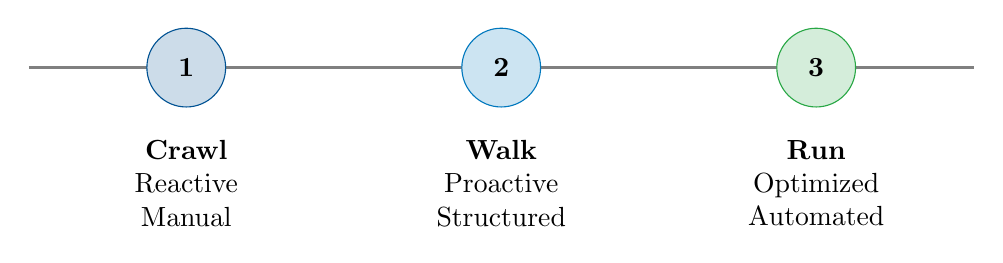
\begin{tikzpicture}
    \draw[thick, gray] (0,0) -- (12,0);
    
    \node[circle, draw=primaryblue, fill=primaryblue!20, minimum size=1cm] at (2,0) {\textbf{1}};
    \node[circle, draw=secondaryblue, fill=secondaryblue!20, minimum size=1cm] at (6,0) {\textbf{2}};
    \node[circle, draw=successgreen, fill=successgreen!20, minimum size=1cm] at (10,0) {\textbf{3}};
    
    \node[align=center, anchor=north] at (2,-0.8) {\textbf{Crawl}\\Reactive\\Manual};
    \node[align=center, anchor=north] at (6,-0.8) {\textbf{Walk}\\Proactive\\Structured};
    \node[align=center, anchor=north] at (10,-0.8) {\textbf{Run}\\Optimized\\Automated};
\end{tikzpicture}
\caption{FinOps Maturity Model: Crawl, Walk, Run}
\end{figure}

\subsection{Required Reading}

\begin{readingbox}
\textbf{Cloud FinOps, 2nd Edition} by Storment \& Fuller
\begin{itemize}[leftmargin=*]
    \item Chapter 9: Building the FinOps Team
    \item Chapter 10: FinOps Culture and Organizational Change
    \item Chapter 11: FinOps Maturity Model
\end{itemize}
\end{readingbox}

\subsection{Phase 1 Assessment}

\begin{assessmentbox}
\textbf{Phase 1 Capstone Project: FinOps Foundation Proposal}\\[0.3cm]
\textbf{Objective:} Develop a comprehensive proposal for establishing or enhancing a FinOps practice in your organization.\\[0.3cm]
\textbf{Requirements:}
\begin{enumerate}[leftmargin=*]
    \item Executive summary articulating the business case for FinOps
    \item Current state assessment including maturity evaluation
    \item Proposed organizational structure and team composition
    \item Implementation roadmap with milestones and success metrics
    \item Quick-win identification for first 90 days
\end{enumerate}
\textbf{Format:} 10--15 page proposal with executive presentation deck\\
\textbf{Evaluation Criteria:} Business case clarity, technical accuracy, organizational feasibility, actionability
\end{assessmentbox}

% ============================================================================
% CHAPTER 3: PHASE 2 - IMPLEMENTATION
% ============================================================================
\chapter{Phase 2: Platform Implementation}
\thispagestyle{fancy}

\begin{tcolorbox}[colback=secondaryblue!5, colframe=secondaryblue, title=Phase Overview]
\textbf{Duration:} 6 Weeks \hfill \textbf{Primary Texts:} Platform-specific guides\\[0.3cm]
\textbf{Objective:} Implement FinOps practices on primary cloud platforms with hands-on tool proficiency
\end{tcolorbox}

\section{Module 2.1: AWS FinOps Implementation}

\duration{Weeks 5--6} \hfill \difficulty{Intermediate}

\subsection{Learning Objectives}

\begin{objectivebox}
Upon completing this module, participants will be able to:
\begin{itemize}[leftmargin=*]
    \item Design AWS account structures optimized for cost management
    \item Implement comprehensive tagging strategies using AWS Tag Editor and Resource Groups
    \item Configure AWS Cost Explorer, Budgets, and Cost Anomaly Detection
    \item Analyze and recommend Reserved Instance and Savings Plan purchases
    \item Execute rightsizing using AWS Compute Optimizer
    \item Build custom cost allocation reports using Cost and Usage Reports (CUR)
\end{itemize}
\end{objectivebox}

\subsection{Topics Covered}

\subsubsection{AWS Account Structure for FinOps}

\begin{itemize}[leftmargin=*]
    \item \textbf{AWS Organizations:} Multi-account strategy with consolidated billing
    \item \textbf{Organizational Units (OUs):} Hierarchical grouping by environment, business unit, or function
    \item \textbf{Service Control Policies (SCPs):} Guardrails for cost governance
    \item \textbf{Cost Allocation Tags:} User-defined and AWS-generated tags for granular tracking
\end{itemize}

\subsubsection{AWS Cost Management Tools}

\begin{table}[H]
\centering
\begin{tabularx}{\textwidth}{>{\bfseries}l X}
\toprule
\textbf{Tool} & \textbf{Purpose} \\
\midrule
Cost Explorer & Interactive cost visualization and analysis \\
AWS Budgets & Threshold-based alerts and automated actions \\
Cost Anomaly Detection & ML-powered spend anomaly identification \\
Cost and Usage Report (CUR) & Detailed, granular billing data export \\
Compute Optimizer & Rightsizing recommendations for EC2, EBS, Lambda \\
Trusted Advisor & Best practice recommendations including cost optimization \\
Savings Plans & Flexible commitment-based discount management \\
\bottomrule
\end{tabularx}
\caption{AWS Cost Management Tool Suite}
\end{table}

\subsubsection{AWS Cost Optimization Techniques}

\textbf{Compute Optimization:}
\begin{itemize}[leftmargin=*]
    \item EC2 rightsizing based on CloudWatch metrics and Compute Optimizer
    \item Spot Instance integration for fault-tolerant workloads
    \item Graviton (ARM) migration for improved price-performance
    \item Auto Scaling optimization for demand-based scaling
\end{itemize}

\textbf{Storage Optimization:}
\begin{itemize}[leftmargin=*]
    \item S3 Intelligent-Tiering for automatic access-based placement
    \item EBS volume rightsizing and GP3 migration
    \item Lifecycle policies for data archival
\end{itemize}

\textbf{Data Transfer Optimization:}
\begin{itemize}[leftmargin=*]
    \item VPC endpoint implementation to reduce NAT Gateway costs
    \item CloudFront caching to minimize origin data transfer
    \item Regional data locality strategies
\end{itemize}

\subsection{Required Reading}

\begin{readingbox}
\textbf{AWS FinOps Simplified} by Peter Chung
\begin{itemize}[leftmargin=*]
    \item Chapter 1--3: AWS FinOps Foundations
    \item Chapter 4--6: Cost Visibility and Allocation on AWS
    \item Chapter 7--9: AWS Cost Optimization Strategies
    \item Chapter 10--12: Reserved Instances and Savings Plans
\end{itemize}
\textbf{Efficient Cloud FinOps} by San Miguel Sánchez \& Obando García
\begin{itemize}[leftmargin=*]
    \item AWS-specific sections throughout
\end{itemize}
\end{readingbox}

\subsection{Hands-On Labs}

\begin{labbox}
\textbf{Lab 2.1a: AWS Cost Visibility Setup}\\[0.3cm]
\textbf{Activities:}
\begin{enumerate}[leftmargin=*]
    \item Configure Cost and Usage Report with Athena integration
    \item Create custom Cost Explorer saved reports
    \item Set up AWS Budgets with action thresholds
    \item Enable and tune Cost Anomaly Detection monitors
    \item Implement a tagging compliance dashboard
\end{enumerate}
\end{labbox}

\begin{labbox}
\textbf{Lab 2.1b: AWS Cost Optimization Execution}\\[0.3cm]
\textbf{Activities:}
\begin{enumerate}[leftmargin=*]
    \item Run Compute Optimizer analysis and implement top 5 recommendations
    \item Analyze EC2 utilization and execute rightsizing
    \item Evaluate Savings Plan coverage and model purchase scenarios
    \item Identify and terminate unused resources (EBS, EIPs, snapshots)
    \item Implement S3 lifecycle policies for cost optimization
\end{enumerate}
\end{labbox}

% ============================================================================
% Module 2.2
% ============================================================================
\section{Module 2.2: Azure FinOps Implementation}

\duration{Weeks 7--8} \hfill \difficulty{Intermediate}

\subsection{Learning Objectives}

\begin{objectivebox}
Upon completing this module, participants will be able to:
\begin{itemize}[leftmargin=*]
    \item Design Azure subscription and management group hierarchies for cost governance
    \item Implement Azure tagging strategies with Azure Policy enforcement
    \item Configure Azure Cost Management + Billing for visibility and alerting
    \item Leverage Azure Advisor for optimization recommendations
    \item Analyze Reserved Instance opportunities using Azure portal and APIs
    \item Implement Azure Hybrid Benefit for Windows and SQL workloads
\end{itemize}
\end{objectivebox}

\subsection{Topics Covered}

\subsubsection{Azure Resource Hierarchy}

\begin{itemize}[leftmargin=*]
    \item \textbf{Management Groups:} Root-level hierarchy for policy inheritance
    \item \textbf{Subscriptions:} Billing and access control boundary
    \item \textbf{Resource Groups:} Logical containers for related resources
    \item \textbf{Tags:} Metadata for cost allocation and governance
\end{itemize}

\subsubsection{Azure Cost Management + Billing}

\begin{table}[H]
\centering
\begin{tabularx}{\textwidth}{>{\bfseries}l X}
\toprule
\textbf{Capability} & \textbf{Description} \\
\midrule
Cost Analysis & Multi-dimensional cost exploration with custom views \\
Budgets & Threshold-based alerts with automated actions \\
Exports & Scheduled cost data exports to storage accounts \\
Recommendations & Azure Advisor integration for optimization suggestions \\
Power BI Integration & Advanced visualization and reporting \\
\bottomrule
\end{tabularx}
\caption{Azure Cost Management Capabilities}
\end{table}

\subsubsection{Azure-Specific Optimization Strategies}

\textbf{Azure Hybrid Benefit:}
\begin{itemize}[leftmargin=*]
    \item Bring existing Windows Server licenses to Azure (up to 85\% savings)
    \item SQL Server license mobility for Azure SQL
    \item Linux Hybrid Benefit for RHEL and SUSE subscriptions
\end{itemize}

\textbf{Azure Reserved Instances:}
\begin{itemize}[leftmargin=*]
    \item Virtual Machines: 1-year and 3-year terms
    \item Azure SQL Database and Managed Instance
    \item Cosmos DB reserved capacity
    \item Azure Synapse Analytics and Databricks
\end{itemize}

\subsection{Required Reading}

\begin{readingbox}
\textbf{FinOps Handbook for Microsoft Azure} by Maulik Soni
\begin{itemize}[leftmargin=*]
    \item Complete book coverage (all chapters)
\end{itemize}
\textbf{Efficient Cloud FinOps} by San Miguel Sánchez \& Obando García
\begin{itemize}[leftmargin=*]
    \item Azure-specific sections throughout
\end{itemize}
\end{readingbox}

\subsection{Hands-On Labs}

\begin{labbox}
\textbf{Lab 2.2: Azure Cost Management Implementation}\\[0.3cm]
\textbf{Activities:}
\begin{enumerate}[leftmargin=*]
    \item Configure Azure Cost Management with custom scopes and views
    \item Create budgets with email and Action Group alerts
    \item Implement Azure Policy for tag enforcement
    \item Generate Reserved Instance recommendations and model savings
    \item Configure scheduled exports to storage account with Power BI integration
\end{enumerate}
\end{labbox}

% ============================================================================
% Module 2.3
% ============================================================================
\section{Module 2.3: Multi-Cloud FinOps Strategies}

\duration{Weeks 9--10} \hfill \difficulty{Intermediate}

\subsection{Learning Objectives}

\begin{objectivebox}
Upon completing this module, participants will be able to:
\begin{itemize}[leftmargin=*]
    \item Design unified tagging taxonomies across AWS, Azure, and GCP
    \item Implement normalized cost reporting for multi-cloud environments
    \item Evaluate and select third-party FinOps tools for multi-cloud visibility
    \item Develop cloud-agnostic cost optimization frameworks
    \item Create cross-cloud chargeback and showback models
\end{itemize}
\end{objectivebox}

\subsection{Topics Covered}

\subsubsection{Multi-Cloud Tagging Strategy}

Consistent tagging across clouds enables unified cost allocation:

\begin{table}[H]
\centering
\begin{tabularx}{\textwidth}{l X X X}
\toprule
\textbf{Tag Category} & \textbf{AWS} & \textbf{Azure} & \textbf{GCP} \\
\midrule
Cost Center & CostCenter & costCenter & cost\_center \\
Environment & Environment & environment & env \\
Application & Application & application & app \\
Owner & Owner & owner & owner \\
Project & Project & project & project \\
\bottomrule
\end{tabularx}
\caption{Sample Multi-Cloud Tagging Taxonomy}
\end{table}

\subsubsection{Third-Party FinOps Tools}

\begin{itemize}[leftmargin=*]
    \item \textbf{Apptio Cloudability:} Enterprise-grade multi-cloud cost management
    \item \textbf{CloudHealth by VMware:} Multi-cloud visibility and governance
    \item \textbf{Spot by NetApp:} Optimization automation and container cost management
    \item \textbf{Kubecost:} Kubernetes-specific cost allocation and optimization
    \item \textbf{Vantage:} Developer-focused cloud cost intelligence
    \item \textbf{Infracost:} Infrastructure-as-code cost estimation
\end{itemize}

\subsubsection{GCP FinOps Fundamentals}

While this curriculum emphasizes AWS and Azure, GCP fundamentals include:

\begin{itemize}[leftmargin=*]
    \item \textbf{Organization and Folder Hierarchy:} Resource organization for governance
    \item \textbf{Labels:} GCP equivalent of tags for cost allocation
    \item \textbf{Cloud Billing:} Budget alerts, exports, and BigQuery integration
    \item \textbf{Committed Use Discounts:} Flexible and resource-based commitments
    \item \textbf{Recommender:} ML-powered optimization recommendations
\end{itemize}

\subsection{Required Reading}

\begin{readingbox}
\textbf{Efficient Cloud FinOps} by San Miguel Sánchez \& Obando García
\begin{itemize}[leftmargin=*]
    \item Chapter 4--6: Multi-Cloud Cost Management
    \item Chapter 7--9: Unified Reporting and Dashboards
    \item Chapter 10--12: Optimization Across Clouds
\end{itemize}
\end{readingbox}

\subsection{Phase 2 Assessment}

\begin{assessmentbox}
\textbf{Phase 2 Capstone Project: Platform Implementation Portfolio}\\[0.3cm]
\textbf{Objective:} Demonstrate proficiency in implementing FinOps on your primary cloud platform(s).\\[0.3cm]
\textbf{Requirements:}
\begin{enumerate}[leftmargin=*]
    \item Complete documentation of implemented cost visibility solution
    \item Before/after cost analysis showing optimization impact
    \item Tagging compliance report with governance policy documentation
    \item Reserved Instance/Savings Plan purchase recommendation with ROI analysis
    \item Dashboard screenshots and configuration documentation
\end{enumerate}
\textbf{Format:} Technical portfolio with evidence of implementation\\
\textbf{Evaluation Criteria:} Implementation completeness, measurable savings, documentation quality
\end{assessmentbox}

% ============================================================================
% CHAPTER 4: PHASE 3 - SPECIALIZATION
% ============================================================================
\chapter{Phase 3: Specialization and Depth}
\thispagestyle{fancy}

\begin{tcolorbox}[colback=accentorange!5, colframe=accentorange, title=Phase Overview]
\textbf{Duration:} 6 Weeks \hfill \textbf{Primary Texts:} FinOps for Snowflake, Practical FinOps\\[0.3cm]
\textbf{Objective:} Develop specialized expertise in platform-specific optimization and automation
\end{tcolorbox}

\section{Module 3.1: Snowflake FinOps}

\duration{Weeks 11--12} \hfill \difficulty{Intermediate}

\subsection{Learning Objectives}

\begin{objectivebox}
Upon completing this module, participants will be able to:
\begin{itemize}[leftmargin=*]
    \item Explain Snowflake's unique pricing model (compute credits, storage, data transfer)
    \item Implement visibility into Snowflake cost drivers using ACCOUNT\_USAGE views
    \item Optimize warehouse configurations for cost-performance balance
    \item Design governance policies for Snowflake resource usage
    \item Apply FinOps practices to Snowflake Cortex and AI/ML workloads
\end{itemize}
\end{objectivebox}

\subsection{Topics Covered}

\subsubsection{Snowflake Pricing Model Deep Dive}

Snowflake's pricing differs fundamentally from IaaS providers:

\begin{table}[H]
\centering
\begin{tabularx}{\textwidth}{>{\bfseries}l X l}
\toprule
\textbf{Component} & \textbf{Pricing Basis} & \textbf{Optimization Focus} \\
\midrule
Compute & Credits per second (warehouse runtime) & Warehouse sizing, suspension, clustering \\
Storage & TB per month (compressed) & Data lifecycle, cloning, zero-copy \\
Data Transfer & Per GB egress & Regional placement, caching \\
Cloud Services & Credits (>10\% of compute) & Query optimization, metadata \\
Serverless & Credits per execution & Task efficiency \\
\bottomrule
\end{tabularx}
\caption{Snowflake Pricing Components}
\end{table}

\subsubsection{Snowflake Cost Visibility}

\begin{itemize}[leftmargin=*]
    \item \textbf{ACCOUNT\_USAGE Schema:} Historical usage views (WAREHOUSE\_METERING\_HISTORY, QUERY\_HISTORY)
    \item \textbf{ORGANIZATION\_USAGE Schema:} Cross-account visibility for enterprise deployments
    \item \textbf{Resource Monitors:} Budget thresholds with suspend/notify actions
    \item \textbf{Tagging and Labels:} Object-level metadata for cost allocation
\end{itemize}

\subsubsection{Snowflake Optimization Strategies}

\textbf{Warehouse Optimization:}
\begin{itemize}[leftmargin=*]
    \item Right-size warehouses based on query complexity patterns
    \item Configure auto-suspend (30 seconds to 10 minutes based on workload)
    \item Implement multi-cluster warehouses for concurrency scaling
    \item Separate warehouses by workload type (ETL, BI, ad-hoc)
\end{itemize}

\textbf{Query Optimization:}
\begin{itemize}[leftmargin=*]
    \item Leverage result caching and data caching
    \item Optimize clustering keys for large tables
    \item Use materialized views for frequently accessed aggregations
    \item Implement query profiling and optimization reviews
\end{itemize}

\subsection{Required Reading}

\begin{readingbox}
\textbf{FinOps for Snowflake} by Ravi Kumar, Natarajan, \& Bhardwaj
\begin{itemize}[leftmargin=*]
    \item Complete book coverage (all chapters)
    \item Special focus on Snowflake Cortex and AI/ML cost management (newest content)
\end{itemize}
\end{readingbox}

\subsection{Hands-On Lab}

\begin{labbox}
\textbf{Lab 3.1: Snowflake Cost Optimization}\\[0.3cm]
\textbf{Activities:}
\begin{enumerate}[leftmargin=*]
    \item Create a Snowflake cost visibility dashboard using ACCOUNT\_USAGE views
    \item Implement Resource Monitors for budget controls
    \item Analyze warehouse utilization and implement rightsizing
    \item Configure auto-suspend and auto-resume policies
    \item Identify and optimize top 10 most expensive queries
\end{enumerate}
\end{labbox}

% ============================================================================
% Module 3.2
% ============================================================================
\section{Module 3.2: FinOps Automation Fundamentals}

\duration{Weeks 13--14} \hfill \difficulty{Intermediate--Advanced}

\subsection{Learning Objectives}

\begin{objectivebox}
Upon completing this module, participants will be able to:
\begin{itemize}[leftmargin=*]
    \item Design automated cost optimization workflows using cloud-native tools
    \item Implement SQL-driven cost analysis and reporting pipelines
    \item Build automated anomaly detection and alerting systems
    \item Create Infrastructure-as-Code templates with cost guardrails
    \item Develop automated remediation playbooks for common cost issues
\end{itemize}
\end{objectivebox}

\subsection{Topics Covered}

\subsubsection{Automation Patterns in FinOps}

\begin{table}[H]
\centering
\begin{tabularx}{\textwidth}{>{\bfseries}l X X}
\toprule
\textbf{Pattern} & \textbf{Description} & \textbf{Example Implementation} \\
\midrule
Scheduled Analysis & Regular cost reporting and optimization scans & Lambda/Functions with CloudWatch/Timer triggers \\
Event-Driven Response & React to cost anomalies or threshold breaches & SNS/Event Grid triggers with remediation functions \\
Policy Enforcement & Prevent non-compliant resource creation & AWS SCPs, Azure Policy, OPA/Gatekeeper \\
Self-Healing & Automatic remediation of identified issues & Auto-tagging, unused resource cleanup \\
\bottomrule
\end{tabularx}
\caption{FinOps Automation Patterns}
\end{table}

\subsubsection{SQL-Driven Cost Analysis}

Leveraging billing data exports (AWS CUR, Azure Exports, GCP BigQuery) for advanced analysis:

\begin{itemize}[leftmargin=*]
    \item Athena/BigQuery/Synapse queries for granular cost exploration
    \item Trend analysis and forecasting using SQL window functions
    \item Anomaly detection using statistical methods in SQL
    \item Custom allocation and chargeback calculations
\end{itemize}

\subsubsection{Infrastructure-as-Code Cost Integration}

\begin{itemize}[leftmargin=*]
    \item \textbf{Infracost:} Pre-commit cost estimation for Terraform
    \item \textbf{AWS CloudFormation Guard:} Policy-as-code for cost controls
    \item \textbf{Azure Policy:} Deny policies for expensive resources
    \item \textbf{OPA/Conftest:} Universal policy engine for IaC validation
\end{itemize}

\subsection{Required Reading}

\begin{readingbox}
\textbf{Practical FinOps} by Mohamed Labouardy
\begin{itemize}[leftmargin=*]
    \item Part I: Visibility and Accountability Automation
    \item Part II: Multi-Cloud Workflows
    \item Chapter X: SQL Queries for Cost Analysis (with sample queries)
\end{itemize}
\end{readingbox}

\subsection{Hands-On Lab}

\begin{labbox}
\textbf{Lab 3.2: Automated Cost Optimization Pipeline}\\[0.3cm]
\textbf{Activities:}
\begin{enumerate}[leftmargin=*]
    \item Set up Athena/BigQuery integration with billing data
    \item Write SQL queries for common cost analysis patterns
    \item Build a serverless function for unused resource detection
    \item Implement automated tagging compliance remediation
    \item Create a cost estimation pipeline for IaC deployments
\end{enumerate}
\end{labbox}

% ============================================================================
% Module 3.3
% ============================================================================
\section{Module 3.3: AI/ML for FinOps}

\duration{Weeks 15--16} \hfill \difficulty{Advanced}

\subsection{Learning Objectives}

\begin{objectivebox}
Upon completing this module, participants will be able to:
\begin{itemize}[leftmargin=*]
    \item Apply machine learning techniques for cost forecasting
    \item Implement AI-powered anomaly detection systems
    \item Use LLMs for automated optimization recommendations
    \item Evaluate AI/ML FinOps tools and their appropriate use cases
    \item Design feedback loops for continuous learning optimization
\end{itemize}
\end{objectivebox}

\subsection{Topics Covered}

\subsubsection{ML-Powered Cost Forecasting}

\begin{itemize}[leftmargin=*]
    \item Time series forecasting: ARIMA, Prophet, DeepAR
    \item Feature engineering from billing and usage data
    \item Model training and validation strategies
    \item Forecast accuracy metrics and continuous improvement
\end{itemize}

\subsubsection{AI-Driven Anomaly Detection}

\begin{itemize}[leftmargin=*]
    \item Statistical methods: Z-score, IQR, moving averages
    \item Machine learning: Isolation Forest, Autoencoders
    \item Cloud-native solutions: AWS Cost Anomaly Detection, Azure Anomaly Detector
    \item Alert tuning to balance sensitivity and noise
\end{itemize}

\subsubsection{LLMs for FinOps Automation}

\begin{itemize}[leftmargin=*]
    \item Natural language interfaces for cost queries
    \item Automated report generation and summarization
    \item Recommendation explanation and contextualization
    \item Conversational FinOps assistants
\end{itemize}

\subsection{Required Reading}

\begin{readingbox}
\textbf{Practical FinOps} by Mohamed Labouardy
\begin{itemize}[leftmargin=*]
    \item Part III: AI and LLM Integration for Cost Optimization
    \item Chapter Y: Building AI-Powered FinOps Workflows
\end{itemize}
\end{readingbox}

\subsection{Phase 3 Assessment}

\begin{assessmentbox}
\textbf{Phase 3 Capstone Project: Automation Implementation}\\[0.3cm]
\textbf{Objective:} Design and implement an automated FinOps workflow.\\[0.3cm]
\textbf{Options (choose one):}
\begin{enumerate}[leftmargin=*]
    \item \textbf{Cost Optimization Bot:} Automated detection and remediation of common waste patterns
    \item \textbf{Forecasting System:} ML-powered cost forecasting with accuracy validation
    \item \textbf{Snowflake Governance:} Automated warehouse management and query optimization
    \item \textbf{IaC Cost Pipeline:} Pre-deployment cost estimation with policy enforcement
\end{enumerate}
\textbf{Deliverables:} Working implementation, documentation, demo recording\\
\textbf{Evaluation Criteria:} Technical implementation, automation coverage, business impact potential
\end{assessmentbox}

% ============================================================================
% CHAPTER 5: PHASE 4 - SCALING
% ============================================================================
\chapter{Phase 4: Organizational Scaling}
\thispagestyle{fancy}

\begin{tcolorbox}[colback=successgreen!5, colframe=successgreen, title=Phase Overview]
\textbf{Duration:} 4--8 Weeks \hfill \textbf{Primary Text:} Scaling Cloud FinOps\\[0.3cm]
\textbf{Objective:} Develop capabilities to scale FinOps practices across enterprise organizations
\end{tcolorbox}

\section{Module 4.1: FinOps Organizational Design}

\duration{Weeks 17--18} \hfill \difficulty{Advanced}

\subsection{Learning Objectives}

\begin{objectivebox}
Upon completing this module, participants will be able to:
\begin{itemize}[leftmargin=*]
    \item Design FinOps organizational structures for different enterprise contexts
    \item Develop executive communication strategies for FinOps initiatives
    \item Create governance frameworks that balance agility with cost control
    \item Build stakeholder engagement programs for cross-functional adoption
    \item Measure and communicate FinOps program ROI
\end{itemize}
\end{objectivebox}

\subsection{Topics Covered}

\subsubsection{Enterprise FinOps Organizational Models}

\begin{table}[H]
\centering
\begin{tabularx}{\textwidth}{>{\bfseries}l X}
\toprule
\textbf{Model} & \textbf{Characteristics} \\
\midrule
Cloud Center of Excellence (CCoE) & Centralized governance, distributed execution, strong policy framework \\
Federated FinOps & BU-level FinOps teams with central coordination and standards \\
Platform Engineering & FinOps embedded in internal platform team offerings \\
Finance-Led & Strong finance leadership with engineering partnerships \\
\bottomrule
\end{tabularx}
\caption{Enterprise FinOps Organizational Models}
\end{table}

\subsubsection{The Piggy-Bank Framework}

From \textit{Scaling Cloud FinOps}, the Piggy-Bank framework provides a structured approach to cost governance:

\begin{itemize}[leftmargin=*]
    \item \textbf{P}olicies: Define cost-related policies and standards
    \item \textbf{I}ncentives: Align organizational incentives with cost efficiency
    \item \textbf{G}overnance: Establish review and approval processes
    \item \textbf{G}uardrails: Implement preventive controls
    \item \textbf{Y}ield: Measure and optimize returns on cloud investment
\end{itemize}

\subsubsection{Executive Sponsorship and Communication}

\begin{itemize}[leftmargin=*]
    \item Building the business case for FinOps investment
    \item Executive dashboard design and KPI selection
    \item Board-level reporting frameworks
    \item Crisis communication during cost overruns
\end{itemize}

\subsection{Required Reading}

\begin{readingbox}
\textbf{Scaling Cloud FinOps} by Kanumuri \& Zeier
\begin{itemize}[leftmargin=*]
    \item Part I: FinOps Organizational Design
    \item Part II: The Piggy-Bank Framework
    \item Chapter X: Executive Engagement and Communication
\end{itemize}
\textbf{Cloud FinOps, 2nd Edition} by Storment \& Fuller
\begin{itemize}[leftmargin=*]
    \item Chapter 12: Connecting FinOps to Other Frameworks
    \item Chapter 13: Sustainability and FinOps
\end{itemize}
\end{readingbox}

% ============================================================================
% Module 4.2
% ============================================================================
\section{Module 4.2: FinOps Maturity and Continuous Improvement}

\duration{Weeks 19--20} \hfill \difficulty{Advanced}

\subsection{Learning Objectives}

\begin{objectivebox}
Upon completing this module, participants will be able to:
\begin{itemize}[leftmargin=*]
    \item Assess organizational FinOps maturity using the FinOps Foundation framework
    \item Design maturity advancement roadmaps with measurable milestones
    \item Implement continuous improvement processes for FinOps practices
    \item Develop training and enablement programs for organizational adoption
    \item Create community of practice structures for knowledge sharing
\end{itemize}
\end{objectivebox}

\subsection{Topics Covered}

\subsubsection{FinOps Maturity Assessment}

The FinOps Foundation defines maturity across multiple capability domains:

\begin{enumerate}[leftmargin=*]
    \item \textbf{Understanding Cloud Usage and Cost:} Cost allocation, visibility, reporting
    \item \textbf{Performance Tracking and Benchmarking:} KPIs, unit economics, trend analysis
    \item \textbf{Real-Time Decision Making:} Anomaly detection, alerts, rapid response
    \item \textbf{Cloud Rate Optimization:} Commitments, spot usage, pricing optimization
    \item \textbf{Cloud Usage Optimization:} Rightsizing, architectural efficiency
    \item \textbf{Organizational Alignment:} Governance, accountability, culture
\end{enumerate}

\subsubsection{Maturity Advancement Strategies}

\begin{table}[H]
\centering
\begin{tabularx}{\textwidth}{>{\bfseries}c X X}
\toprule
\textbf{Level} & \textbf{Characteristics} & \textbf{Advancement Focus} \\
\midrule
Crawl & Reactive, manual, limited visibility & Establish basic visibility and reporting \\
Walk & Proactive, structured processes, growing automation & Expand coverage, standardize practices \\
Run & Optimized, automated, cultural integration & Continuous improvement, innovation \\
\bottomrule
\end{tabularx}
\caption{Maturity Level Progression Strategies}
\end{table}

\subsubsection{Training and Enablement Programs}

\begin{itemize}[leftmargin=*]
    \item Role-based training curriculum design
    \item Self-service learning resources and documentation
    \item Certification pathways (FinOps Certified Practitioner, FinOps Certified Professional)
    \item Gamification and incentive programs
\end{itemize}

\subsection{Required Reading}

\begin{readingbox}
\textbf{Scaling Cloud FinOps} by Kanumuri \& Zeier
\begin{itemize}[leftmargin=*]
    \item Part III: Maturity Models and Assessment
    \item Part IV: Organizational Adoption Patterns
\end{itemize}
\end{readingbox}

% ============================================================================
% Module 4.3
% ============================================================================
\section{Module 4.3: Advanced Governance and Sustainability}

\duration{Weeks 21--24} \hfill \difficulty{Advanced}

\subsection{Learning Objectives}

\begin{objectivebox}
Upon completing this module, participants will be able to:
\begin{itemize}[leftmargin=*]
    \item Design comprehensive cloud governance frameworks
    \item Integrate sustainability metrics into FinOps practices (GreenOps)
    \item Implement multi-cloud governance strategies
    \item Develop compliance and audit frameworks for cloud financial management
    \item Create vendor management strategies for cloud cost optimization
\end{itemize}
\end{objectivebox}

\subsection{Topics Covered}

\subsubsection{Comprehensive Cloud Governance}

\begin{itemize}[leftmargin=*]
    \item Policy framework design (preventive, detective, responsive)
    \item Approval workflows and exception management
    \item Compliance monitoring and reporting
    \item Risk management integration
\end{itemize}

\subsubsection{GreenOps: Sustainability in FinOps}

\begin{itemize}[leftmargin=*]
    \item Carbon footprint visibility (AWS Carbon Footprint, Azure Carbon Dashboard)
    \item Sustainability-aware optimization decisions
    \item Renewable energy region selection
    \item Efficiency metrics (carbon per transaction, energy per compute hour)
\end{itemize}

\subsubsection{Vendor and Contract Management}

\begin{itemize}[leftmargin=*]
    \item Enterprise Discount Program (EDP) negotiation strategies
    \item Multi-cloud vendor management
    \item License optimization and compliance
    \item Partner and reseller relationship management
\end{itemize}

\subsection{Final Program Assessment}

\begin{assessmentbox}
\textbf{Program Capstone: Enterprise FinOps Transformation Plan}\\[0.3cm]
\textbf{Objective:} Develop a comprehensive FinOps transformation plan for a real or simulated enterprise environment.\\[0.3cm]
\textbf{Requirements:}
\begin{enumerate}[leftmargin=*]
    \item \textbf{Current State Assessment:} Maturity evaluation across all capability domains
    \item \textbf{Target State Vision:} 18-month FinOps maturity goals
    \item \textbf{Organizational Design:} Team structure, roles, and governance model
    \item \textbf{Technology Roadmap:} Tool selection and implementation plan
    \item \textbf{Quick Wins:} 90-day action plan with measurable savings targets
    \item \textbf{Metrics Framework:} KPIs, dashboards, and reporting cadence
    \item \textbf{Change Management:} Training, communication, and adoption strategy
    \item \textbf{Sustainability Integration:} GreenOps considerations
\end{enumerate}
\textbf{Format:} Comprehensive strategy document (30--50 pages) with executive presentation\\
\textbf{Evaluation:} Strategic coherence, technical depth, organizational feasibility, measurability
\end{assessmentbox}

% ============================================================================
% CHAPTER 6: SUPPLEMENTARY MATERIALS
% ============================================================================
\chapter{Supplementary Materials}

\section{Recommended Reading Schedule}

\begin{table}[H]
\centering
\small
\begin{tabularx}{\textwidth}{c X X}
\toprule
\textbf{Week} & \textbf{Primary Reading} & \textbf{Supplementary Reading} \\
\midrule
1--2 & Cloud FinOps (2e), Ch. 1--6 & FinOps Foundation online resources \\
3--4 & Cloud FinOps (2e), Ch. 7--11 & Efficient Cloud FinOps, Ch. 1--3 \\
5--6 & AWS FinOps Simplified (full) & AWS Well-Architected Framework \\
7--8 & FinOps Handbook for Azure (full) & Azure Well-Architected Framework \\
9--10 & Efficient Cloud FinOps, Ch. 4--12 & GCP Cloud Architecture Framework \\
11--12 & FinOps for Snowflake (full) & Snowflake documentation \\
13--14 & Practical FinOps, Part I--II & Cloud provider automation docs \\
15--16 & Practical FinOps, Part III & AI/ML platform documentation \\
17--20 & Scaling Cloud FinOps (full) & FinOps Foundation case studies \\
21--24 & Cloud FinOps (2e), Ch. 12--14 & Industry sustainability reports \\
\bottomrule
\end{tabularx}
\caption{Weekly Reading Schedule}
\end{table}

\section{FinOps Certification Alignment}

This curriculum prepares participants for FinOps Foundation certifications:

\begin{table}[H]
\centering
\begin{tabularx}{\textwidth}{>{\bfseries}l X c}
\toprule
\textbf{Certification} & \textbf{Coverage} & \textbf{Curriculum Alignment} \\
\midrule
FinOps Certified Practitioner (FOCP) & Foundational FinOps knowledge & Phases 1--2 \\
FinOps Certified Professional (FCP) & Advanced practitioner skills & Phases 3--4 \\
FinOps Certified Engineer (FCE) & Technical implementation & Phases 2--3 \\
\bottomrule
\end{tabularx}
\caption{Certification Alignment Matrix}
\end{table}

\section{Key Performance Indicators (KPIs)}

\subsection{Cost Efficiency Metrics}

\begin{itemize}[leftmargin=*]
    \item \textbf{Effective Savings Rate:} (On-demand equivalent - Actual cost) / On-demand equivalent
    \item \textbf{Commitment Coverage:} Committed spend / Total eligible spend
    \item \textbf{Waste Rate:} Unused resources cost / Total cost
    \item \textbf{Rightsizing Opportunity:} Potential savings from rightsizing / Total compute cost
\end{itemize}

\subsection{Operational Metrics}

\begin{itemize}[leftmargin=*]
    \item \textbf{Tagging Compliance:} Tagged resources / Total resources
    \item \textbf{Budget Accuracy:} |Forecast - Actual| / Actual
    \item \textbf{Anomaly Detection Rate:} Detected anomalies / Total anomalies
    \item \textbf{Mean Time to Optimization:} Average time from identification to remediation
\end{itemize}

\subsection{Business Value Metrics}

\begin{itemize}[leftmargin=*]
    \item \textbf{Cost per Unit:} Cloud cost / Business unit (transaction, user, revenue dollar)
    \item \textbf{Cloud ROI:} (Business value generated - Cloud cost) / Cloud cost
    \item \textbf{Engineering Efficiency:} Value delivered / Engineering cloud spend
\end{itemize}

\section{Tool Ecosystem Reference}

\subsection{Cloud-Native Tools}

\begin{table}[H]
\centering
\begin{tabularx}{\textwidth}{l X X X}
\toprule
\textbf{Category} & \textbf{AWS} & \textbf{Azure} & \textbf{GCP} \\
\midrule
Cost Visibility & Cost Explorer, CUR & Cost Management + Billing & Cloud Billing, BigQuery \\
Budgets/Alerts & AWS Budgets & Azure Budgets & Cloud Billing Budgets \\
Optimization & Compute Optimizer & Azure Advisor & Recommender \\
Commitments & Savings Plans, RIs & Reserved Instances & CUDs \\
Anomaly Detection & Cost Anomaly Detection & Anomaly Detector & Built-in alerts \\
\bottomrule
\end{tabularx}
\caption{Cloud-Native FinOps Tool Comparison}
\end{table}

\subsection{Third-Party Tools}

\begin{table}[H]
\centering
\begin{tabularx}{\textwidth}{>{\bfseries}l X}
\toprule
\textbf{Tool} & \textbf{Primary Use Case} \\
\midrule
Apptio Cloudability & Enterprise multi-cloud cost management \\
CloudHealth (VMware) & Multi-cloud governance and optimization \\
Spot by NetApp & Container and compute optimization automation \\
Kubecost & Kubernetes cost allocation and optimization \\
Vantage & Developer-focused cost intelligence \\
Infracost & Infrastructure-as-code cost estimation \\
Densify & ML-powered resource optimization \\
nOps & AWS cost optimization automation \\
\bottomrule
\end{tabularx}
\caption{Third-Party FinOps Tools}
\end{table}

\section{Glossary of Key Terms}

\begin{description}[leftmargin=!,labelwidth=4cm]
    \item[Chargeback] Allocating cloud costs directly to consuming business units
    \item[Showback] Displaying cloud costs to teams without direct billing impact
    \item[Unit Economics] Cost metrics normalized by business units (cost per user, transaction, etc.)
    \item[Rightsizing] Adjusting resource capacity to match actual workload requirements
    \item[Reserved Instance] Pre-purchased compute capacity at discounted rates
    \item[Savings Plan] Flexible commitment for compute usage with discounted pricing
    \item[Committed Use Discount] GCP equivalent of reserved capacity pricing
    \item[Spot Instance] Unused capacity available at steep discounts with interruption risk
    \item[Tagging] Metadata attached to resources for cost allocation and governance
    \item[FinOps Maturity] Organizational capability level: Crawl, Walk, Run
\end{description}

% ============================================================================
% APPENDIX
% ============================================================================
\appendix

\chapter{Assessment Rubrics}

\section{Phase 1 Capstone Rubric}

\begin{table}[H]
\centering
\begin{tabularx}{\textwidth}{X c c c c}
\toprule
\textbf{Criterion} & \textbf{Excellent (4)} & \textbf{Good (3)} & \textbf{Adequate (2)} & \textbf{Needs Work (1)} \\
\midrule
Business Case Clarity & Compelling & Clear & Basic & Unclear \\
Technical Accuracy & Comprehensive & Accurate & Minor errors & Significant gaps \\
Organizational Fit & Tailored & Appropriate & Generic & Misaligned \\
Actionability & Immediately executable & Feasible & Conceptual & Impractical \\
Documentation Quality & Professional & Clear & Adequate & Poor \\
\bottomrule
\end{tabularx}
\caption{Phase 1 Assessment Rubric}
\end{table}

\section{Program Capstone Rubric}

\begin{table}[H]
\centering
\begin{tabularx}{\textwidth}{X c c c c}
\toprule
\textbf{Criterion} & \textbf{Excellent (4)} & \textbf{Good (3)} & \textbf{Adequate (2)} & \textbf{Needs Work (1)} \\
\midrule
Strategic Coherence & Integrated vision & Aligned & Fragmented & Disconnected \\
Technical Depth & Expert-level & Proficient & Basic & Superficial \\
Measurability & Comprehensive KPIs & Key metrics & Limited & No metrics \\
Change Management & Complete strategy & Good plan & Acknowledged & Ignored \\
Innovation & Novel approaches & Best practices & Standard & Outdated \\
Presentation Quality & Executive-ready & Professional & Adequate & Unprepared \\
\bottomrule
\end{tabularx}
\caption{Program Capstone Assessment Rubric}
\end{table}

\chapter{Sample Lab Worksheets}

\section{Cloud Spend Discovery Worksheet}

\begin{table}[H]
\centering
\begin{tabularx}{\textwidth}{X X}
\toprule
\textbf{Discovery Item} & \textbf{Finding} \\
\midrule
Total Monthly Cloud Spend & \$ \_\_\_\_\_\_\_\_\_\_\_\_ \\
Number of Accounts/Subscriptions & \_\_\_\_\_\_\_\_\_\_\_\_ \\
Top 5 Services by Cost & 1. \_\_\_\_ 2. \_\_\_\_ 3. \_\_\_\_ 4. \_\_\_\_ 5. \_\_\_\_ \\
Tagging Coverage Percentage & \_\_\_\_\_\_\_\% \\
Reserved Instance Coverage & \_\_\_\_\_\_\_\% \\
Identified Waste (Unused Resources) & \$ \_\_\_\_\_\_\_\_\_\_\_\_ \\
Current FinOps Maturity Level & Crawl / Walk / Run \\
\bottomrule
\end{tabularx}
\caption{Cloud Spend Discovery Worksheet Template}
\end{table}

% ============================================================================
% END MATTER
% ============================================================================

\chapter*{Acknowledgments}
\addcontentsline{toc}{chapter}{Acknowledgments}

This curriculum draws upon the collective wisdom of the FinOps community, with special recognition to the authors of the core texts that form the foundation of this program:

\begin{itemize}[leftmargin=*]
    \item J.R. Storment and Mike Fuller for their foundational work on Cloud FinOps
    \item Alfonso San Miguel Sánchez and Jose Obando García for practical multi-cloud guidance
    \item Peter Chung for AWS-specific expertise
    \item Maulik Soni for Azure implementation knowledge
    \item Y.V. Ravi Kumar, Velu Natarajan, and Parag Bhardwaj for Snowflake specialization
    \item Mohamed Labouardy for automation and AI integration insights
    \item Sasi Kanumuri and Matthew Zeier for organizational scaling strategies
\end{itemize}

Additional thanks to the FinOps Foundation for establishing the professional framework that guides this discipline.

\vfill

\begin{center}
\textit{Cloud FinOps Professional Curriculum}\\
\textit{Version 1.0 --- 2025 Edition}
\end{center}

\end{document}
